%%%%%%%%%%%%%%%%%%% vorlage.tex %%%%%%%%%%%%%%%%%%%%%%%%%%%%%
%
% LaTeX-Vorlage zur Erstellung von Projekt-Dokumentationen
% im Fachbereich Informatik der Hochschule Trier
%
% Basis: Vorlage svmono des Springer Verlags
%
%%%%%%%%%%%%%%%%%%%%%%%%%%%%%%%%%%%%%%%%%%%%%%%%%%%%%%%%%%%%%

\documentclass[envcountsame,envcountchap, deutsch]{i-studis}

\let\thempfootnote\thefootnote
\usepackage[LGR,T1]{fontenc}
\usepackage[utf8]{inputenc}
\usepackage{makeidx}         	% Index
\usepackage{multicol}        	% Zweispaltiger Index
 \newcommand{\textgreek}[1]{\begingroup\fontencoding{LGR}\selectfont#1\endgroup}

%\usepackage[bottom]{footmisc}	% Erzeugung von Fu�noten

%%-----------------------------------------------------
%\newif\ifpdf
%\ifx\pdfoutput\undefined
%\pdffalse
%\else
%\pdfoutput=1
%\pdftrue
%\fi
%%--------------------------------------------------------
%\ifpdf
\usepackage[pdftex]{graphicx}
\usepackage{epstopdf}
\usepackage[pdftex,plainpages=false]{hyperref}
%\else
%\usepackage{graphicx}
%\usepackage[plainpages=false]{hyperref}
%\fi

%%-----------------------------------------------------
\usepackage{color}				% Farbverwaltung
%\usepackage{ngerman} 			% Neue deutsche Rechtsschreibung
\usepackage[english, ngerman]{babel}

%%-----------------------------------------------------
% Unterscheidung für Umlaute Windows-Mac
%%-----------------------------------------------------

%\usepackage[latin1]{inputenc} 	% Ermöglicht Umlaute-Darstellung
\usepackage[utf8]{inputenc}  	% Ermöglicht Umlaute-Darstellung unter Linux (je nach verwendetem Format)

%-----------------------------------------------------
\usepackage{listings} 			% Code-Darstellung
\lstset
{
	basicstyle=\scriptsize, 	% print whole listing small
	keywordstyle=\color{blue}\bfseries,
								% underlined bold black keywords
	identifierstyle=, 			% nothing happens
	commentstyle=\color{red}, 	% white comments
	stringstyle=\ttfamily, 		% typewriter type for strings
	showstringspaces=false, 	% no special string spaces
	framexleftmargin=7mm, 
	tabsize=3,
	showtabs=false,
	frame=single, 
	rulesepcolor=\color{blue},
	numbers=left,
	linewidth=146mm,
	xleftmargin=8mm
}

\usepackage{textcomp} 			% Celsius-Darstellung
\usepackage{amssymb,amsfonts,amstext,amsmath}	% Mathematische Symbole
\usepackage[german, ruled, vlined]{algorithm2e}
\usepackage[a4paper]{geometry} % Andere Formatierung
\usepackage{bibgerm}
\usepackage{array}
\hyphenation{Ele-men-tar-ob-jek-te  ab-ge-tas-tet Aus-wer-tung House-holder-Matrix Le-ast-Squa-res-Al-go-ri-th-men} 		% Weitere Silbentrennung bei Bedarf angeben
\setlength{\textheight}{1.1\textheight}
\pagestyle{myheadings} 			% Erzeugt selbstdefinierte Kopfzeile
\makeindex 						% Index-Erstellung


%--------------------------------------------------------------------------
\begin{document}
%------------------------- Titelblatt -------------------------------------
\title{Titel der Arbeit}
\project{Zulassungsarbeit zum Master-Fernstudium}
%--------------------------------------------------------------------------
\supervisor{Titel Vorname Name} 		% Betreuer der Arbeit
\author{Vorname Nachname}							% Autor der Arbeit
\address{Ort,} 							% Im Zusammenhang mit dem Datum wird hinter dem Ort ein Komma angegeben
\submitdate{Abgabedatum} 				% Abgabedatum
%\begingroup
%  \renewcommand{\thepage}{title}
%  \mytitlepage
%  \newpage
%\endgroup
\begingroup
  \renewcommand{\thepage}{Titel}
  \mytitlepage
  \newpage
\endgroup
%--------------------------------------------------------------------------
\frontmatter 
%--------------------------------------------------------------------------
\kurzfassung

%% deutsch
\paragraph*{}

Neuronale Netze sind in den vergangenen Jahren ein wesentlicher Bestandteil von Forschung und Anwendung in der Medizin geworden.

Die vorliegende Arbeit stellt einige solcher Netze sowie deren theoretischen Unterbauten vor.

Hierzu wird im ersten Teil zunächst die Fachlichkeit zusammengefasst, die Grundlage künstlicher neuronaler Netze ist: Das biologische Neuron mit seinen komplexen biochemischen Vorgängen, die Signalverarbeitung und -weiterleitung in einem Netz aus Nervenzellen ermöglichen.

Darauf aufbauend bietet der zweite Teil eine Einführung in das mathematischen Gerüst des McCulloch-Pitts-Neurons und Rosenblatt-Perzeptrons, zwei frühe Modelle künstlicher Neuronen, die für Forschung und Wissenschaft einen wesentlichen Beitrag geleistet haben.
Anwendungsbeispiele beleuchten die unterschiedlichen Eigenschaften hinsichtlich Statik des McCulloch-Pitts-Neurons und Anpassungsfähigkeit des Rosenblatt-Perzeptrons.

Im dritten Teil werden einige wegweisende Architekturen und Algorithmen künstlicher neuronaler Netze aufgeführt, darunter  Backpropagation sowie Faltungsoperationen, die den tiefen Netzen zu eigen sind, die heutzutage in der Medizin angewendet werden, wo sie grosse Erfolge vorweisen können.

Einige dieser Erfolge werden im vierten Teil vorgestellt.
Ausgewählte Forschungsarbeiten und -Ergebnisse aus dem Gesundheitswesen wie Gesundheitswirtschaft, der Pharmafoschung sowie der Diagnostik und Therapie bezeugen die Leistungsfähigkeit künstlicher neuronaler Netze.
 			% Kurzfassung Deutsch/English
\tableofcontents 						% Inhaltsverzeichnis
%--------------------------------------------------------------------------
\mainmatter                        		% Hauptteil (ab hier arab. Seitenzahlen)
%--------------------------------------------------------------------------
% Die Kapitel werden in separaten .tex-Dateien abgelegt und hier eingebunden.
\input{chapters/Einführung}
\chapter{Das Neuron}

\section{Struktur einer Nervenzelle}

\begin{figure}[h]
	\centering
		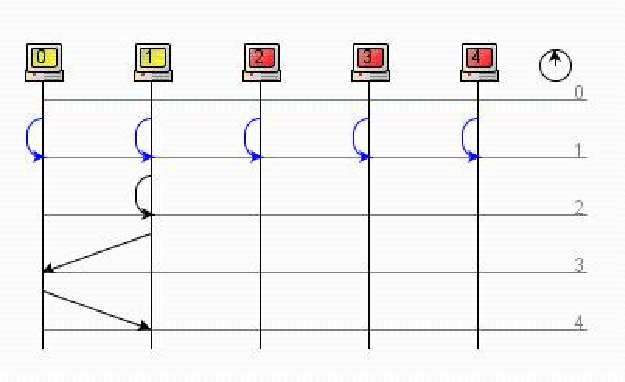
\includegraphics{images/p1ReadSeq.pdf}
\caption{Aufbau einer Nervenzelle}
\small
 1. Die Dendriten\footnotemark[1] leiten
 afferente\footnotemark[2] Signale zum 
 2. Soma\footnotemark[3], dem Zellkörper.
 3. Das Axon\footnotemark[4] leitet ein
 efferentes\footnotemark[5] Nervensignal über präsynaptische Endigungen (Axonterminale) an (häufig weit 
 entfernte\footnotemark[6]) 
 Effektoren\footnotemark[7]
 wie Muskeln und Drüsen oder nachgeschaltete Neuronen 
 weiter\footnotemark[8] {[SD07:42, Abs. d2]}

\end{figure}

\footnotetext[1]{``\textgreek{δένδρον} (dendrón)`` (altgriechisch): Baum}
\footnotetext[2]{``afferre`` (lat.): herbeibringen, melden, bringen}
\footnotetext[3]{``\textgreek{σῶμα} (sõma)`` (altgriechisch): Körper}
\footnotetext[4]{``axon`` (lat.): Achse}
\footnotetext[5]{``efferre`` (lat.): hinaustragen, mitnehmen}
\footnotetext[6]{Axone können sich im menschlichen Körper über Entfernungen von bis zu über 1m ausstrecken {[BCP18:28, Abs. 2]}}
\footnotetext[7]{``efficere`` (lat.): bewirken, hervorbringen} 
\footnotetext[8]{in diesem Fall empfangen postsynaptische Rezeptoren an den Dendriten des nachgeschalteten Neurons ein Signal und der beschriebene Prozess wiederholt sich. Bildlich können wir uns Effektoren als Endglied der Signalübertragung vorstellen, auch wenn hier wieder interzelluläre Vorgänge stattfinden. Vgl. ``neuromuskuläre Endplatte`` {[BCP18:127, Abs. 3]}} 

Die eingehende Schnittstelle eines Neurons sind seine \textbf{Dendriten}: Baumförmige Fortsätze\footnotemark[9], die um das \textbf{Soma}\footnotemark[10] herum gelagert sind.
Diese Dendritenbäume [BCP18:47] fungieren \textit{postsynaptisch} und empfangen afferente Signale in Form von Neurotransmittern [Eil19:61, ``Synapsen``].
Diese werden von Rezeptoren, die sich an den Enden der Dendriten befinden, aufgenommen.
Oft stehen tausende Neuronen in Verbindung mit den Dendriten eines einzelnen Neurons\footnotemark[10] [SD07, S .42].\\


Die \textbf{Dendriten} leiten Signale weiter an das Soma.
In der Zelle befindet sich das durch die \textit{Neuronenmembran}\footnotemark[11] von der Umgebung getrennte \textit{Zytosol}, eine salzige, wässrige Flüssigkeit mit einem hohen Anteil von Kalium [BCP18:29, ``Das Soma``]\footnotemark[12].
In dem Zytosol eingebettet sind weitere subzelluläre Strukturen mit eigener Membranbegrenzung, die \textit{Zellorganellen} [SD07:8, Abs. 2].\\
Für die weitere Betrachtung ist für uns die Zellmembran und der \textit{transmembranale Transport} von Ionen\footnotemark[13] zur Änderung des Membranpotenzials interessant. In der Nähe des \textbf{Axonhügels}\footnotemark[14] entspringt das \textbf{Axon}, welches in einer ``salzigen extrazellulären Flüssigkeit mit hoher Leitfähigkeit`` [PCB18:61, Abs. 1]\footnotemark[15] liegt.
Hier entscheidet sich, ob das Neuron Informationen weiterleitet: Die Summation der durch die postsynaptischen Endigungen eingehenden Signale kann eine Depolarisation\footnotemark[16] der Membran an dieser Stelle [Eil19:61, ``Soma``] über einen gewissen \textbf{Schwellenwert} bewirken, so das ein \textbf{Aktionspotenzial} ausgelöst wird [BCP18, p.142 f.], was in den präsynaptischen Endigungen die \textbf{Exozytose}\footnotemark[17] verursacht.

\footnotetext[9]{einzelne selten länger als 2mm {[BCP18:28, Abs. 2]}. Längere Dendriten finden sich an den kortikalen Pyramidenzellen mit einer Länge von 1 cm {[Eil19:58, ``Polarisierung``]} }
\footnotetext[10]{ oder \textit{Perikaryon} [RK18:58, ``Aufbau``]. Bezeichnet den Zellkörper und das Stoffwechselzentrum des Neurons mit der eine Grösse von ca. 20 μm [BCP18:29]. Zum Vergleich: ein menschliches Haar hat einen Durchmesser von ca. 70 μm, kleine Bakterien bis zu 20 μm.}
\footnotetext[10]{das menschliche Gehirn besitzt mindestens $10^{11}$ Neuronen [KSJ+13:175, Abs. 2]}
\footnotetext[11]{Membrandicke ca. 5 nm {[FE19:66, letzter Absatz linke Spalte]}}
\footnotetext[12]{ vgl. Ionenkonzentrationen in Tabelle~\ref{tab:ionenkonzentration}}
\footnotetext[13]{hier: der Austausch von Ionen zwischen dem intra- und extrazellulären Raum durch Kanäle und Pumpen. Ion: Ein elektrisch geladenes Atom oder Molekül.}
\footnotetext[14]{ca. 20 - 50 µm vom Soma entfernt [Jon19:77, ``Ort der Aktionspotenzialinitiation``]}
\footnotetext[15]{{[BCP18:43, Abs. 1]}, führt das Axon metaphorisch mit einer Telefonleitung zusammen. Aufgrund der signalempfangenden Eigenschaften und der dünnen Spitzen der Dendriten liegt auch der Vergleich mit ``Antennen`` nahe {[BCP18:28, Abs. 2]}}
\footnotetext[16]{\textit{Depolarisation} bezeichnet die Verringerung des Membranpotenzials von einem negativen Wert auf einen weniger negativen oder gar einen positiven Wert {[RHN+16:812 ``Neurotransmitter und ihre Rezeptoren``]}}
\footnotetext[17]{bezeichnet den Stofftransport aus der Zelle heraus. In den nachfolgenden Abschnitten wird hierdrauf noch näher eingegangen.}


\section{Das Ruhepotenzial}
\subsection{Die Entdeckung bioelektrischer Ströme}

Im Jahr 1912 veröffentlichte der deutsche Physiologe \textit{Julius Bernstein} (1839-1917) Erkenntnisse seiner elektrophysiologischen Studien in dem Buch ``\textit{Elektrobiologie - Die Lehre von den elektrischen Vorgängen im Organismus auf moderner Grundlage dargestellt}``.
In dem Kapitel ``Membrantheorie`` [Ber12:87] greift er das Postulat seiner Arbeit ``Untersuchungen zur Thermodynamik der bioelektrischen Ströme`` [Ber02] auf. Bereits 1902 von ihm veröffentlicht, lieferte die Theorie die erste plausible physikalisch-chemische Erklärung bioelektrischer Phänomene [Sey06:5. ``4 Membrane Theory (1902)``]:
In Zellen befindet sich eine elektrolytische Flüssigkeit, die von einer für bestimmte Ionen permeablen Membran umgeben ist. Diese Membran besitzt eine Potenzialdifferenz\footnotemark[18].


In den darauffolgenden Jahren und Jahrzehnten haben zahlreiche Forschungen die Theorie bestätigt: Wir wissen heute, dass die ungleiche Ionenverteilung in der intrazellulären und extrazellulären Flüssigkeit zusammen mit der Permeabilität der Membran für die Entstehung eines Membranpontenzials verantwortlich ist. Im folgenden wollen wir diese Zusammenhänge betrachten, um ein besseres Verständnis für die Signalweiterleitung von Neuronen zu erlangen, die in den nachfolgenden Abschnitten untersucht werden.

\footnotetext[18]{
vgl. {[Ber12:92 f.]} sowie {[Ber02:542]}:
 ``Denken wir uns, dass diese Elektrolyte aus dem Querschnitt der Fibrillen ungehindert in die umgebende Flüssigkeit diffundieren, wahrend sie am Längsschnitt durch die lebende Sarkoplasmahaut daran gehindert werden, well sie für ein Ion derselben, z. B. für das Anion ($PO^-_4$ u. s. w.), mehr oder weniger impermeabel ist, so entstünde auf der Oberfläche der Fibrille eine elektrische Doppelschicht, welche nach innen negative, nach aussen positive Spannung besitzen würde.``
}


\subsection{Ionenkonzentrationen und Membranspannungen}

Ein Neuron weist \textit{in Ruhe}\footnotemark[19] eine ungleiche Ionenverteilung zwischen der durch die Zellmembran getrennten intrazellulären Flüssigkeit (IZF: Zytosol) und der extrazellulären Flüssigkeit (EZF) auf.
In der IZF befinden sich mehr positiv geladene Natrium-Ionen ($Na^+$), und im EZF mehr positiv geladene Kalium- und Calcium-Ionen ($Ka^+$ und $Ca^{2+}$) sowie mehr negativ geladene Chlorid-Ionen ($Cl^-$).

\footnotetext[19]{
 vgl. \textbf{Mempranpotenzial}: ``die Spannung an der Nervenzellmembran zu einem beliebigen Zeitpunkt`` {[BCP18:70, ``Ionen als Grundlage des Ruhepotenzials``]}; \textbf{Ruhepotenzial}: ``the electrical potential across the membrane in the absence of signaling`` {[KSJ+13:126]}
}

{\renewcommand{\arraystretch}{1.5}%
\begin{table} %[hbtp]
 \centering
 \begin{tabular}{l | c | c | c }
  \textbf{Ion} & \textbf{Konzentration EZF (mmol/l)} & \textbf{Konzentration IZF (mmol/l)} & \textbf{Verhältnis} \\
  \hline
  $K^+$      & 5 & 100 & 1 : 20 \\
  $Na^+$     & 150 & 15 & 10:1 \\
  $Ca^{2+}$  & 2 & 0,0002 & 10000 : 1 \\
  $Cl^-$     & 150 & 13 & 11,5 : 1 \\
 \end{tabular}
 \caption{Ionenkonzentration eines Neurons in Ruhe (nach {[BCP18:75, Abb. 3.15]})}
 \label{tab:ionenkonzentration}
\end{table}


Das Membranpotenzial des Neurons wird durch die Verteilung von Ionen in der IZF und EZF bestimmt: In der Membran befinden sich \textbf{Ionenkanäle}, von denen viele \textit{selektiv permeabel}\footnotemark[20] sind.
Neben den Ionenkanälen existieren auch \textbf{Ionenpumpen}\footnotemark[21], die für die Aufrechterhaltung der Ionenverteilung zuständig sind: die $Ca^{2+}$- und $Na^+$-$K^+$-ATPasen sorgen dafür, dass im Neuron laufend  $Ca^{2+}$ und $Na^+$ aus und $K^+$ in die Zelle gepumpt wird [SD07:44]).
Zusammen mit den selektiv permeablen Ionenkanälen entstehen so die Ionenkonzentrationen in Tabelle~\ref{tab:ionenkonzentration}.\\

\footnotetext[20]{
 von ``\textit{permeare}`` (lat.) durchwandern. Diese Kanäle sind nur für bestimmte Ionen durchlässig (\textit{ionenselektiv}). Kaliumkanäle sind durchlässig für $K^+$-Ionen, Natriumkanäle durchlässig für $Na^+$-Ionen usw. (vgl. {[BCP18:66., Abs. 3]}).
 Sie können über Änderungen in der Umgebung des Neurons geöffnet oder geschlossen werden, was auch als \textbf{Gating} bezeichnet wird (vgl. {[KSJ+13:108, 2. Abs. rechte Spalte]})
}
\footnotetext[21]{
 sog. \textbf{ATPasen}, Kurzform für \textit{Adenosintriphosphasen}: Enzyme, die ATP in ADP und Phosphat aufspalten {[SD07:26, Abs. 2]}) \textbf{QUELLE}
}


Wenn auf das Neuron kein \textit{postsynaptisches Potenzial} (PSP) wirkt und das Neuron keinen Impuls abgibt, liegt das Ruhepotenzial $V_r$ der Zelle zwischen -70 mV und -90 mV\footnotemark[22]: Das Zytosol weist entlang der Membranoberfläche im IZF eine negative Ladung auf\footnotemark[23].
Diese \textit{Membranspannung} $V_m$ wird durch eine ungleiche Ionenverteilung bewirkt [FE19:66, ``Diffusionspotenzial – elektrische Spannung über der Zellmembran``]), verursacht durch die Ladung der Teilchen im IZF und EZF in Membrannähe\footnotemark[24].


\begin{figure}[h]
 \centering
 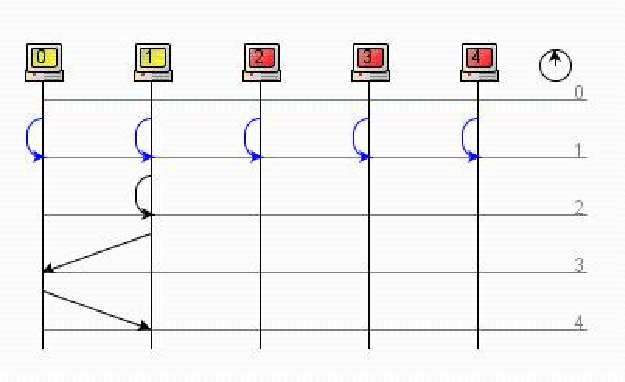
\includegraphics{images/p1ReadSeq.pdf}
 \caption{Ionenverteilung im Zytosol und der EZF}
 \small
 Aufgrund der elektrostatischen Anziehungskraft ziehen sich Anionen und Kationen\footnotemark[25] in der Nähe der Membran gegenseitig an, es kommt zu einer negativen Spannung in Membrannähe (zwischen -70 mV -90 mV in Ruhe).
\end{figure}



\footnotetext[22]{
vgl. {[SD07:47, Tafel 2.3 A.1]}. \textit{Bear et al.} geben -65 mV an (1 mV = 0,001 V), also wird von einer 40-mal höheren Ionenpermeabilität für $K^+$ gegenüber $Na^+$ ausgegangen ({[BCP18:74, Exkurs 3.2] und [BCP18:70, ``Ionen als Grundlage des Ruhepotenzials``]})
}
\footnotetext[23]{
 vgl. {[BCP18:61, Abs.3]}. Das Membranpotenzial $V_m$ ergibt sich als die Differenz der Spannungen $V_{IZF}$ und $V_ezf$, wobei $V_{IZF}$ die Spannung im IZF und $V_{EZF}$ die Spannung im EZF ist. $V_r$ ist dann gleich zu $V_{IZF}$: Wenn die Zelle in Ruhe ist, wird die Spannung im EZF als $0$ definiert {[KSJ+13:127, rechte Spalte, Abs. 2]}.
}
\footnotetext[24]{
 ``Die negativen Ladungen im Inneren des Neurons und die positiven Ladungen außerhalb des Neurons ziehen sich in Richtung Zellmembran gegenseitig an, {[...]} Dementsprechend ist die negative Nettoladung im Inneren der Zelle nicht gleichmäßig im Cytosol verteilt, sondern an der Innenseite der Membran lokalisiert.`` {[BCP18:72, Punkt 2]}
}
\footnotetext[25]{
 \textit{Anion}: negativ geladenes Ion; \textit{Kation}: positiv geladenes Ion
}


In Ruhe ist die Leitfähigkeit der Membran für $Na^+$ gering, für $K^+$ hingegen hoch [SD07:44 f.].
$K^+$-Ionen folgen ihrem Konzentrationsgradienten\footnotemark[26] und gelangen über die Ionenkanäle in den EZF, bis die Potenzialdifferenz entlang der Neuronenmembran ausströmende $K^+$-Ionen zurückhält: Wenn diese Differenz den Konzentrationsgradienten für $K^+$ kompensiert, erhält man das \textbf{Gleichgewichtspotenzial}\footnotemark[27].
Das Wert des Membranpotenzial nähert sich dem Wert des Gleichgewichtspotenzials desjenigen Ions an, für den die Membran besonders permeabel ist [KSJ+13:145, Ende] $(S1.1)$.\\
Das Gleichgewichtspotenzial lässt sich für individuelle Ionen mit der Nernst-Gleichung\footnotemark[28] ermitteln:\\

\textit{Bear et al.} definieren [BCP18:74, Exkurs 3.2]:
\begin{equation}
E_{Ion} = 2,303  \times \begin{matrix} RT \\ \hline zF \end{matrix} \times log_{10} \times \begin{matrix} [Ion]_{EZF} \\ \hline [Ion]_{IZF} \end{matrix}
\label{eq:gl-nernst}
\end{equation}

wobei

  {\renewcommand{\arraystretch}{1.5}%
\begin{table} %[hbtp]
 \centering
 \begin{tabular}{l |l }
  \textbf{Variable / Konstante} & \textbf{Bedeutung}  \\
  \hline
  $E_{ion}$            & Gleichgewichtspotenzial für das jeweilige Ion \\
  $R$                  & Gaskonstante \\
  $T$                  & absolute Temperatur \\
  $z$                  & Ladungszahl des Ions \\
  $F$                  & Faraday-Konstante \\
  $[Ion]_{EZF}$        & Ionenkonzentration \textbf{ausserhalb} der Zelle \\
  $[Ion]_{IZF}$        & Ionenkonzentration \textbf{innerhalb} der Zelle \\
 \end{tabular}
 \caption{Nomenklatur Nernst-Gleichung\footnotemark[29]}
 \label{tab:nernstkonstanten}
\end{table}




\footnotetext[26]{
unter der Diffusion (``\textit{diffundere}`` (lat.): zerstreuen, ausbreiten) von Molekülen versteht man ihr Bestreben, entlang eines Konzentrationsgradienten (auch: Konzentrationsgefälles) einen Ausgleich der Konzentrationsunterschiede zu erreichen. Moleküle in hoher Konzentration diffundieren dann in die Bereiche mit niedriger Konzentration: In den hier betrachteten Beispielen diffundieren bspw. $K^+$-Ionen, bis das Gleichgewichtspotenzial erreicht ist.
}
\footnotetext[27]{
vgl. {[BCP18:72 f.] sowie [SD07:44 f.]}. \textit{Kandel et al.} schreiben hierzu:
``the equilibrium potential of any ion that is present on both sides of a membrane permeable to that ion`` {[KSJ+13:130, letzter Abs., linke Spalte]}
}
\footnotetext[28]{
vgl. {[FE19:67, ``Nernst-Gleichung``]}.
\textit{Walther Nernst} (1864 - 1941) war ein deutscher Physiker und Chemiker und gehört zu den Begründern der physikalischen Chemie. Er formulierte das \textbf{Nernst-Theorem}, auch bekannt als \textbf{Dritter Hauptsatz der Thermodynamik}. 1920 erhielt er den Chemie-Nobelpreis in Anerkennung seiner Arbeit auf dem Gebiet der Thermochemie.
}
\footnotetext[29]{
 $E$ steht für \textit{Equilibrium}: ``Gleichgewicht`` (lat. aequus ``gleich``, libra lat. ``Waage/Gewicht``); \textit{Faraday-Konstante}: elektrische Ladung eines Mols einfach geladener Ionen; 1 Mol = $6.02214076e10^{23}$ Teilchen
}



Für eine Körpertemperatur von 37° lässt sich die Nernst-Gleichung für das Gleichgewichtspotenzial $E_K$ wie folgt vereinfachen:

\begin{equation}
 E_{K} = 61,54 mV  \times log_{10} \begin{matrix} [K^+]_{EZF} \\ \hline [K^+]_{IZF} \end{matrix}
 \label{eq:gl-nernst-reduced-start}
\end{equation}


Mit den Werten aus Tabelle~\ref{tab:ionenkonzentration}  ergibt sich somit


\begin{equation}
E_{K} = 61,54 mV  \times log_{10} \begin{matrix} 1 \\ \hline 20 \end{matrix} = -80 mV
\label{eq:gl-nernst-reduced-end}
\end{equation}


Wie wir oben gesehen haben, liegt $V_r$ zwischen -70 mV und - 90mV. Wie können wir jetzt auf $(S1.1)$ schliessen, also dass das Ruhepotenzial durch die Membranpermeabilität von $K^+$ bestimmt wird, wenn $V_r = -70 mV$, aber $E_K = -80 mV$, und die Membran auch noch für andere Ionen wie bspw. $Na^+$ selektiv permeabel ist\footnotemark[30]? \\
Wäre die Membran nur für $K^+$ permeable, so läge $V_r$ sicher bei $E_k$ [SD07:32 Abs. 4]: Die Nernst-Gleichung kann deshalb nur zur Bestimmung des Membranpotenzials genutzt werden, wenn die Membran nur für ein Ion permeabel ist. Ansonsten ist der erhaltene Wert nur näherungsweise zu verstehen [HS19a:98, linke Spalte, letzter Absatz].\\

Allerdings können wir das Membranpotenzial auch unter Berücksichtigung mehrerer Ionen bestimmen: Ionenkanäle unterstützen einen \textit{passiven Transport} der Ionen zwischen EZF und IZF \textit{entlang} ihres Konzentrationsgefälles [Fro19:30, ``Aktive und passive Transportmechanismen``], während Ionenpumpen, die \textit{entgegen} des Konzentrationsgefälles arbeiten, \textit{aktiv transportieren}\footnotemark[31].
Ionenpumpen sind für die Ionenkonzentrationsgradienten und deren Aufrechterhaltung verantwortlich [BCP18:76 f.]\footnotemark[32].
Um $V_m$ zu berechnen müssen die Ionen mitberücksichtigt werden, für die die Membran permeabel ist. 
Dazu kann die \textbf{Goldman-Gleichung}\footnotemark[33] genutzt werden\footnotemark[34]:

\begin{equation}
V_{r} = \begin{matrix} RT \\ \hline F \end{matrix}  \times ln \begin{matrix}
  P_{Na} \space  \times \space [Na^+]_{EZF} \space + \space P_{K} \space  \times \space [K^+]_{EZF} \space + \space P_{Cl} \space  \times \space [Cl^-]_{IZF}  \\ \hline
  P_{Na} \space  \times [Na^+]_{IZF} \space + \space P_{K} \space  \times \space [K^+]_{IZF} \space + \space P_{Cl} \space  \times \space [Cl^-]_{EZF}
\end{matrix}
\label{eq:gl-goldman}
\end{equation}

\footnotetext[30]{
 vgl. {[BCP18:77 f.] sowie [SD07:44]}: ``Warum ist $E_m$ weniger negativ als $E_K${?}``
}
\footnotetext[31]{
hierfür wird metabolische Energie verbraucht {[Fro19:31, ``Primär aktiver Transport``]}
}
\footnotetext[32]{
es wird ein nicht unwesentlicher Teil von Energie zur Aufrechterhaltung dieser Gradienten verbraucht. Die Natrium-Kalium-Pumpe verbraucht laut \textit{Bear et al.} etwa 70 \% der ATP-Menge, die das Gehirn benötigt. {[BCP18:76, Abs. 1]}
}
\footnotetext[33]{
auch: \textbf{Goldman-Hodgkin-Katz-Gleichung} (GHK-Gleichung) nach David Eliot Goldman (1910 – 1998), Alan Lloyd Hodgkin(1914 - 1998) und Bernard Katz (1911 - 2003).
}
\footnotetext[34]{
 \textit{Silbernagl und Despopoulos} nutzen für die Bestimmung von $V_m$ die fraktionelle Leitfähgkeit der involvierten Ionen und rechnet $V_r = E_K \times f_K + E_{Na}  \times f_{Na} + E_{Cl}  \times f_{Cl}$ {[SD07:32 Gl. 1.21]}
}

\textit{Kandel et al.} stellen hierzu fest, dass eine hohe Konzentration eines einzelnen Ions zusammen mit einer hohen Membranpermeabilität für dieses Ion auch einen größeren Beitrag für $V_r$ leistet\footnotemark[35]\\
Ein weiteres Merkmal der Membran, auf das wir später zurückgreifen werden, ist die \textit{elektrische Leitfähigkeit} $g_{Ion}$; für sie gilt, dass sie proportional zu der Anzahl der offenen Ionenkanäle $N_{Ion}$ ist [BCP18:93, ``Ströme und Leitfähigkeiten in der Membran``].


\section{Das Aktionspotenzial}
\subsection{Die Entdeckung von Reizwellen}

Bereits 1868 hatte Julius Bernstein - knapp 34 Jahre vor seiner Membrantheorie - die Existenz eines Aktionspotenzials vermutet\footnotemark[36] [Sch83:168].

Knapp 80 Jahre nach Bernsteins Beschreibung der ``negativen Schwankungen`` und 50 Jahre nach seiner Membrantheorie führen Hodgkin und Huxley Experimente an Riesenaxonen von Tintenfischen durch. 
Einige Jahre vorher - 1939 - können Curtis und Cole bei ähnlichen Versuchsanordnungen\footnotemark[37] während der Untersuchung von Membraneigenschaften in Folge eines Aktionspotenzials eines sprunghaften Anstieg der Leitfähigkeit der Membran feststellen [CC39:669, Summary].
Hodgkin und Huxley weisen später nach, dass der Aufstrich des Aktionspotenzials mit einer Zunahme von $g_{Na}$ und dem Einstrom von $Na^+$ zusammenhängt, und weiter, dass die Repolarisation der Zellmembran mit einer Zunahme von $g_K$ und einem Ausstrom von $K^+$ zusammenhängt\footnotemark[38].\\
Sie stellen Hypothesen u.a. zu der Refraktärzeit und dem Schwellenwert auf\footnotemark[39] und formulieren ein mathematisches Modell auf Basis des beobachteten Membranverhaltens [HH52:501, Fig. 1.1], heute bekannt als das \textbf{Hodgkin-Huxley-Modell} [Koc99:142 ff.]\footnotemark[40].

\footnotetext[35]{
 ``{[...]} when permeability to one ion is exceptionally high, the Goldman equation reduces to the Nernst equation for that ion.``{[KSJ+13:135, ``Goldman Equation``]}. \textit{Fakler und Eilers} weisen darauf hin, ``dass die Permeabilitäten in komplizierter Weise von der Membranspannung und den Ionenkonzentrationen {[...]} abhängen und sich meist nur näherungsweise bestimmen lassen.`` {[FE19:67, Goldman Gleichung]}.
}
\footnotetext[36]{
 Seine Forschungsarbeit über elektrische Muskel-Nerven-Aktivitäten {[Ber68]} schließt er mit den Worten:
 ``Ich werde im Folgenden diese Welle mit dem Namen 'Reizwelle' bezeichnen, well derjenige Reiz, durch den die Nervenfaser im Centrum Empfindung, im Muskel Zuckung erzeugt, auf das  Innigste mit dieser Welle verknüpft ist. {[...]} Da wir nachgewiesen haben, dass die Reizwelle mit derselben Geschwindigkeit sich fortpflanzt als die Erregung, so können wir die wohlberechtigte Annahme machen, dass die Reizwelle Nichts anderes ist als das Bild des im Nerven ablaufenden Erregungsvorganges.`` {[Ber68:198 f.]}
}
\footnotetext[37]{
 die Experimente wurden an Riesenaxomen von Tintenfischen durchgeführt, die sich für die damals zur Verfügung stehende Technik mit einer Dicke von ca. 1 mm besser eigneten als die im direkten Vergleich geradezu unfassbar winzigen Axone von menschlichen Nervenzellen (Durchmesser ca 1µm {[Jon19:79, Abs. 1]}) ``The large diameter of the axon, 0.5 mm or more, makes it particularly favorable material {[...]}`` {[CC39:650, Abs. 2]}
}
\footnotetext[38]{
 vgl. {[Jon19:75, ``Permeabilitäten``]}, ausserdem {[BCP18:96, ``Das Aktionspotenzial in der Realität``]} sowie {[HH52:530 Fig. 17.]}
}

\subsection{Eigenschaften des Aktionspotenzials}

In Ruhe ist die Ladung in der IZF negativ, in der EZF positiv.
Durch eine schnelle Umkehrung dieser Verhältnisse ist eine Nervenzelle dazu in der Lage, ein \textit{Signal} auszulösen [BCP18:86, ``Einführung``].
Damit solch ein Impuls ausgelöst werden kann, bedarf es eines \textbf{Aktionspotenzials}: Wir wir im folgenden sehen werden, ist die Entstehung eines Aktionspotenzials auf Ionenbewegungen durch Kanäle zurückzuführen, die durch die Veränderung des Membranpotenzials geöffnet oder geschlossen werden [BCP18:96, Abs.4].

 \textit{Kandel et al.} führen 4 wichtige Eigenschaften des Aktionspotenzials auf [KSJ+13: 148, Abs. 2 f.]:
\begin{enumerate}
 \item Es gibt einen \textbf{Schwellenwert} für die Auslösung des Potenzials.
 \item Das Aktionspotenzial ist ein \textbf{Alles-oder-nichts} Ereignis.
 \item Das Aktionspotenzial wird ohne Verlust weitergeleitet.
 \item Nach dem auslösen des Aktionspotenzial kommt es zu einer \textbf{Refraktärzeit} , in der zunächst kein weiteres Aktionspotenzial ausgelöst werden kann (\textbf{absolute Refraktärzeit}), und dann ein stärkeres Signal benötigt wird, um das Aktionspotenzial auszulösen (\textbf{relative Refraktärzeit}).
\end{enumerate}


\subsection{Auslösung eines Aktionspotenzials}

Das Aktionspotenzial wird über das Axon weitergeleitet. Das Axon - die Nervenfaser - besteht aus einem zylindrischen Zytoplasmaschlaucch und ist von einer Plasmamembran umgeben [Jon19:73, ``Elektrischer Signalfluss im biologischen Kabel``].

Die \textbf{Initiationszone} [BCP18:111, Abs. 1] des Aktionspotenzials ist der Axonhügel. Hier findet sich eine besonders dichte Anhäufung von spannungsabhängigen $Na^+$-Kanälen\footnotemark[41], deren Aktivierungskurve um ca. 10 mV zu den negativen Membranpotenzialen verschoben ist, was die Initiierung des Signals begünstigt [Jon19:77, ``Mechanismen der Aktionspotenzialinitiation und ihrer räumlichen Präferenz``)].

Damit ein Aktionspotenzial ausgelöst werden kann, muß die Membran nahe der Initiationszone über ihren \textbf{Schwellenwert} \footnotemark[42] $V_t$ ( > $V_r$ ) depolarisiert werden [BCP18:111, Abs. 1].

\footnotetext[39]{
 Zum Schwellenwert: ``The curves in Figs. 12 and 21 show that the theoretical 'membrane' has a definite threshold when stimulated by a sudden displacement of membrane potential.`` {[HH52:535, ``Threshold``]}; zur Refraktärzeit: ``Acording to our theory, there are two changes resulting from the depolarization during a spike which make the membrane unable to respond to another stimulus until a certain time has elapsed. These are 'inactivation', which reduces the level to which the sodium conductance can be raised by a depolarization, and the delayed rise in potassium conductance, which tends to hold the membrane potential near to the equilibrium value for potassium ions.`` {[HH52:532, ``Refractory Period``]}
}
\footnotetext[40]{
 Für die Erforschungen der Ionen-Mechanismen, die bei der Erregung und Hemmung von Nervenzellmembranen beteiligt sind, erhalten sie 1963 den Nobelpreis für Physiologie oder Medizin, zusammen mit John Carew Eccles (1903 – 1997) {[DMW63]}. Die Relevanz des Modells fassen \textit{Kandel et al.} so zusammen: ``More than a half-century later the Hodgkin-Huxley model stands as the most successful quantitative model in neural science if not in all of biology.`` {[KSJ+13:156, Abs. 2]}
}

 Als Schwellenwert wird das Membranpotenzial bezeichnet, bei dem die Permeabilität für $Na^+$ größer als für $Ka^+$ ist [BCP18:103, ``Schwellenwert``] ($V_r$ ist in Ruhe nahe an $E_K$); $V_t$ liegt bei ca. - 50mV, unabhängig vom Typ des Neurons [Jon19:75].
 Damit sich $V_r$ an $V_t$ nähert, bedarf es einer Erregung der Zelle durch postsynaptische Potenziale [FE19:69 ``Depolarisation`` f.] oder ``eine aus der Umgebung weitergeleitete (elektrotonische) Erregung`` [SD07:46, Abs. 2].

Die Stärke der Erregung der Zelle ist entscheidend für das Auslösen eines Aktionspotenzials. Es muß mehr $Na^+$ in die Zelle einströmen, als $K^+$ aus der Zelle ausströmen kann [FE19:69, rechte Spalte, Abs. 1] (durch die offenen Ruhemembranpotenzialkanäle und Konzentrationsgradientenausgleich der $Na^+$-$K^+$-ATPasen).
Versuche zeigen, daß die Potenzialänderung der Membran in einem Bereich von -80 mV zu -65 mV kaum Änderung bewirkt [BCP18:99, Abs. 2]. $g_{Ka}$ erhöht sich, aber wenn $V_r$ nicht erreicht wird, bleibt es bei dieser ``lokalen Antwort`` [SD07:46, Abs. 2]. Erst eine Depolarisation der Membran hin über diesen Wert (ab -60 mV gehen die Natrium-Kanäle ein den Offen-Zustand über [FE19:69, rechte Spate, Abs. 2]), kann die \textbf{Initiationsphase} [FE19:68, Abschnitt 6.2] des Aktionspotenzials eingeleitet werden: Es öffnen sich mehr Natrium-Kanäle, und durch die negative Ladung der Membran-Innenseite (IZF) gibt es eine starke elektrochemische Triebkraft für $Na^+$-Ionen [BCP18:103, ``Aufstrich``]. Die Triebkraft ist zu diesem Zeitpunkt die Differenz des Membranpotenzials $V_m$ und $E_{Ka}$. Bei $-60 mV$ beträgt die Triebkraft\footnotemark[43]:

 \begin{equation}
  V_m - E_{Na} = -60 mV - 61,54 mV = -121,54 mV
  \label{eq:gl-triebkraft}
 \end{equation}


Da sich $g_{Ka}$ erhöht durch zunehmende Öffnung der Natrium-Kanäle  [Fak19:46, ``Gating von Kationenkanälen`` ff.], strömen aufgrund der hohen Triebraft für $Na^+$ mehr $Na^+$ Ionen in das Zellinnere. Es kommt zu einem \textbf{Rückkopplungseffekt} , denn die zunehmend weniger negative Membranspannung öffnet weitere Natrium-Kanäle, die Leitfähigkeit der Membran wird weiter erhöht und es kommt zu einem exponentiellen Anstieg der $Na^+$-Konzentration in der IZF. Der ``explosionsartige`` Natriumeinstrom bewirkt die Depolarisation der Membranspannung und das Aktionspotenzial wird ausgelöst [FE19:69, ``Depolarisation`` f.].

\footnotetext[41]{
pro Quadratmikrometer (µm²) kann eine Membran viele tausend Natriumkanäle enthalten {[BCP18:99]}
}
\footnotetext[42]{
``das kritische Niveau der Depolarisation, das überschritten werden muss, um ein Aktionspotenzial auszulösen`` {[BCP18:88, Abs. 1]} oder auch ``Erregungsschwelle`` {[FE19:69, ``Depolarisation``]}
}


Die Stärke des Signals selber ist unabhängig von dem Wert, zur überschwelligen Reizung des Neurons geführt hat: Amplitude und Zeitverlauf des Signals im Axon relativ unabhängig von Intensität und Dauer des Reizes [Jon19:75, ``Aktionspotenziale bei überschwelliger Reizung``]. Entweder kommt es zu einem Aktionspotenzial, oder es bleibt bei der o.g. lokalen Antwort. Aus diesem Grund funktionieren Aktionspotenziale nach dem \textbf{``Alles-oder-Nichts-Prinzip``} [BCP18:89, Abs. 1]\footnotemark[44]:

\blockquote{
 ``A fraction of a millivolt can be the difference between a subthreshold stimulus and a stimulus that generates a full-sized action potential.`` [KSJ+13:157, rechte Spalte, Abs. 2]

}

\subsection{Phasen eines Aktionspotenzials}

Die Generierung von Aktionspotenzialen kann entsprechend der zeitlichen Reihenfolge in folgende Phasen eingeteilt werden:

\subsection*{1. Aufstrich}
$Na^+$ gelangt in die Zelle,  $g_{Ka}$  wird erhöht, mehr $Na+$ strömt ein (positiven Rückkoppellung). 
Es kommt zu einer Depolarisation, $V_m$ wächst exponentiell. [SD07:46, Abs. 3]

\subsection*{2. Overshoot}
$V_m$ wird positiv ($> 0 mV$) und nähert sich insgesamt $E_{Na} \sim 60 mV$\footnotemark[45] an [BCP18:105, ``Overshoot``].

\subsection*{3. Repolarisationsphase\footnotemark[46]}
Natriumkanäle werden \textbf{inaktiviert} .
Spannungsabhängige Kaliumkanäle öffnen sich [BCP18 S. 105, ``Fallende Phase``] ca. 1 ms nach Depolarisation [SD07:47, Tafel 2.3 (A.2)], $K^+$-IOnen strömen aufgrund der elektrochemischen Triebkraft in den EZF, das Membranpotential wird wieder negativ\footnotemark[47].

\subsection*{4. Undershoot\footnotemark[48]}
Es kommt zu einem $V_m$, der unter $V_r$ liegt, da $g_{K}$ noch erhöht ist. $V_m$ nähert sich $E_k$ (-80 mV). Ein erhöhte Pumprate der $Na^+$-$K^+$-ATPase\footnotemark[49] kann auch dazu beitragen [SD07:46, Abs. 1].


\footnotetext[43]{
 vgl. {[Fak19:39, ``Das elektrochemische Potenzial`` f.]}
}
\footnotetext[44]{
 ``Im Computerzeitalter bezeichnet man das axonale Aktionspotenzial auch als 'digitales' Signal.`` {[Jon19:75, ``Aktionspotenzial bei überschwelligger Reizung``]}. \tetxit{Frank} bietet eine Übersicht über die Erforschung des Alles-oder-Nichts-Prinzip in [Fra94]. Dort wird \textit{Lucas} erwähnt, der 1905 in {[Luc05]} die Kontraktionen von Muskelfasern unter diesem Gesichtspunkt untersucht hat {[Fra94:210]}
}
\footnotetext[45]{
den es nicht erreicht. Erreicht werden Werte zwischen 0 und +40 mV [BLS19:69, rechte Spalte, Abs. 2]
}
\footnotetext[46]{
auch: Fallende Phase [BCP18 S. 105, ``Fallende Phase``]
}
\footnotetext[47]{
Die Kaliumleitfähigkeit wird ``verzögerter Gleichrichter`` genannt, da sie das ursprüngliche Membranpotenzial - mit Verzögerung - wiederherstellt [BCP 18:103, ``Spannungsabhängige Kaliumkanäle`` f.]
}
\footnotetext[48]{
auch: Nachhyperpolarisation [SD07 S. 46, rechte Spalte, Asb. 1]
}
\footnotetext[49]{
Die $Na^+$-$K^+$-ATPase ``erhält die Ionenkonzentrationsgradienten aufrecht, die für den Fluss von $Na^+$ und $K^+$ durch die Kanäle während des Aktionspotenzials erforderlich sind`` [BCP18:105, Abs. 2]
}

\subsection*{5. Refraktärphase\footnotemark[50]}

- \textit{absolute}: Ca. 2 ms.
nach Auslösen des Aktionspotenzials [BSJ19:70, ``Refraktärzeit`` f.] sind die $Na^+$ Kanäle  \textit{inaktiviert} und dadurch nicht aktivierbar.
Es ist keine Aktionspotenzialbildung möglich [SD07:47, rechte Spalte, Abs. 3].\\
- \textit{relative}: $V_m$ nähert sich weiter $V_r$ an.
Nachdem einige $Na^+$-Kanäle  \textit{deinaktiviert} wurden, ist eine Auslösung des Aktionspotenzials wieder möglich.
Allerdings ist die Reizschwelle erhöht (da $V_m < V_r < V_t$) und ``die Amplitude des auslösbaren Aktionspotenzials ist reduziert`` [BLS19:70  ``Refraktärzeit`` f.]

\subsection{Signalweiterleitung über das Axon}

Kurz nach der Aktionspotenzialbildung befinden sich daran beteiligte Membrane in der Refraktärphase, ihre $Na^+$-Kanäle sind inaktiviert. 
Somit pflanzt sich das Aktionspotenzial nur in eine Richtung fort\footnotemark[51] ( \textit{orthodrome} Fortleitung) [BCP18:106, Abs. 3].
Die Fortleitung geschieht in Richtung der Axonterminal, wo sich die präsynaptischen Endigungen befinden und das elektrische Signal in chemische Signale umgewandelt werden.

\subsection*{Übertragungsgeschwindigkeit}
Ist das Axon - die Nervenfaser - \textbf{marklos} , wird das Signal kontinuierlich weitergeleitet, und die Leitunsggeschwindigkeit ist eher gering ( ca. 1m/s [BLS19:80, Tab.7.1].
Die Leitunsggeschwindigkeit hängt hier direkt von dem Durchmesser der Nervenfaser ab und ist proportional zur Wurzel des Fasseradius. 
Die marklosen Riesenaxone des Tintenfisches erreichen deshalb aufgrund ihrer Größe Leitungsgeschwindigkeiten von bis zu 20 m / s [BLS19:79, ``Aktive Leitungsgeschwindigkeit``].

Im Gegensatz zu marklosen Nervenfasern erreichen \textbf{myelinisierte Axone}  eine höhere Leitungsgeschwindigkeit.
Sie sind gegenüber ihrer Umgebung durch \textbf{Myelinscheiden}  (Membranschichten, die sich bis zu 100 mal [BLS19:79, 7.3.3 Abs. 1] um das Axon wickeln) besser isoliert [SD07:48, rechte Spalte, Abs. 2].
Dadurch wird der Stromfluss verstärkt und die Erregungsleitung erhöht sich [BCP18:109, Abs. 2]. 
Diese Isolierschicht ist ``segmentiert``: Myelinscheiden sind in Abständen von 0,2 - 2mm durch sog.  \textit{Ranvier-Schnürringe} unterbrochem.
Deren Membran besitzt spannungsabhängige $Na^+$-Kanäle [BCP18:109, Abs. 2], die das ankommende elektrische Signal durch die wie oben beschrieben Depolarisierung der einzelnen Segmentabschnitte kontinuierlich weiterleiten - es wird an den Membranabschnitten jeweils ein neues Aktionspotenzial gebildet [SD07:48, rechte Spalte, Abs.2].
Die Weiterleitung in myeliniserten Axonen bezeichnet man deshalb als \textbf{saltatorische} (sprunghafte) Erregungsleitung [BCP18:110, Abs. 1].

\vskip 1.6in

\footnotetext[50]{
 Die Refraktärphase dient u.a. dazu, die Membran vor einer vorzeitigen Neuerregung zu schützen {[BLS19:76, ``Refraktärzeit``]}.
 Hochfrequenten Aktionspotenzialsalven von max. 1000/s sind aufgrund dieser Eigenschaft möglich (vgl. {[SD07:46, Abs. 2] u. [BCP18:89, letzter Absatz]}).
 \textit{Bear et al.} stellen fest: ``Die Frequenz der Aktionspotenziale ist ein Maß für die Stärke des depolarisierenden Stroms``  {[BCP18:89, Abs. 2]} - je stärker der Reiz, desto mehr Aktionspotenziale werden nacheinander abgefeuert (vgl. {[BCP18:90, Abb. 4.3]}).
}
\footnotetext[51]{
  {[BCP18:106, Abs. 3]} verweist auf \textit{antidrome} Fortleitung, die in Experimenten ausgelöst werden kann
}

\pagebreak

\section{Synaptische Übertragung und Integration}

\subsection{Die Entdeckung des Vagusstoff}

Otto Loewi erhielt 1936 den Nobelpreis für Medizin für seine Forschungen an der chemischen Übertragung von Nervenimpulsen. 
1921 konnte er bei einem Experiment mit Froschpräparaten zeigen, daß die Infusionslösung, die für vorher am Vagusnerv bewusst stimulierte Froschherzen genutzt wurde, den Vagusnerv von nachträglich mit dieser Lösung behandelte Froschherzen stimulieren konnte. 
Loewi vermutete in der Lösung eine Substanz, die er ``Vagusstoff`` nannte.
Henry Dale - mit dem sich Loewi den Nobelpreis teilte - konnte diesen Stoff später als \textit{Acetylcholin} identifizieren, ein exzitatorischer Neurotransmitter\footnotemark[52], der bei chemischen Synapsen als Botenstoff zur Signalübertragung beteiligt ist\footnotemark[53].

\subsection{Synaptische Übertragung}\label{synaptischeuebertragung}
Neben elektrischen Synapsen, bei denen der Signalaustausch durch einen direkten Stromfluss über sog.  	extit{gap junctions} und deren ionenleitfähige Verbindungen\footnotemark[54] passiert [BCP18:103], existieren im Gehirn vor allem \textit{chemische Synapsen} [BCP18:118, Abs. 3]: Die Signalweiterleitung im Gehirn erfolgt überwiegend auf chemische Weise [BCP18:121, ``Chemische Synapsen``, Abs.1].

Chemische Synapsen sind nicht direkt miteinander verbunden. 
Zwischen ihnen existiert ein Spalt, der ca. 20-40 nM breit ist [KSJ+13:184, rechte Spalte, Abs. 1], in der sich eine ``Matrix aus extrazellulären Proteinen``\footnotemark[55]  [BCP18:122, Abs.2 f.] befindet, die den Synapsenspalt überbrückt. 
Die Übertragung von Signalen erfolgt über Exozytose: Botenstoffe (\textit{Neurotransmittern}) diffundieren  aus den präsynaptischen Endigungen in diesen Spalt [BCP18:122, Abs.2 f.], und verschiedene Typen von Rezeptoren an den postsynaptischen Endigungen wandeln die Botenstoffe in hemmende oder erregende Signale um, die dann von der postsynaptischen Zelle nach dem Alles-oder-Nichts-Prinzip integriert werden.

Die durch das Aktionspotenzial ausgelöste Depolarisation der Membran an den Axonterminalen bewirkt eine Öffnung spannungsgeladener Calcium-Canäle [KSJ+13:184, rechte Spalte, Abs. 2].
Durch die ungleiche $Ca^{2+}$ Ionenkonzentration zwischen der EZF und IZF (10.000 : 1:Tabelle~\ref{tab:ionenkonzentration}) entsteht eine hohe Triebkraft für $Ca^{2+}$: Nach Gleichung~\ref{eq:gl-nernst} ergibt sich für das Gleichgewichtspotenzial für $Ca^2+$

\begin{equation}
 E_{Ca^{2+}} = 123,08 mV
 \label{eq:gl-eqca2}
\end{equation}

\footnotetext[52]{
 ``[... ]Acetylcholin wirkt erregend an der motorischen Endplatte, aber hemmend an den Schrittmacherzellen des Herzens`` {[HS19c:105, ``Postsynaptische Rezeptoren vermitteln den Transmittereffekt``]}
}
\footnotetext[53]{
 vgl. {[AHH+98]} sowie {[BCP18:119, Exkurs 5.1]}
}
\footnotetext[54]{
\textit{Konnexone} sind Zell-Zell-Verbindungen {[SD07:50, ``Synaptische Übertragung``, Abs. 2]}
}
\footnotetext[55]{
 lies: \textit{extrazelluläre Matrix}. Hierbei handelt sich um den Gewebeanteil im \textit{Interzellularraum}, also der Raum ausserhalb der Zellen: ``The extracellular matrix {[...]} surrounds all connective tissue cells providing mechanical support and physical strength to tissues, organs and the organism as a whole`` {[AHH+98:3, Abs. 2]}
}

\pagebreak

und bei einem Membranpotenzial von $V_m \sim 20 mV$ durch Depolarisation liegt die Triebkraft für $Ca^{2+}$ bei $\sim -100 mV$:

\begin{equation}
 V_m - E_{Ca^{2+}} = 20 mV - 123,08 mV = -103,08 mV
 \label{eq:gl-triebkraftca2}
\end{equation}


Die Calcium-Ionen strömen in das Innere der Zelle und lösen die Exozytose von \textbf{synaptischen Vesikeln}\footnotemark[56] aus, kleine, mit einer Membran von der IZF getrennte Strukturen von etwa 50 nm Durchmesser, die mit Neurotransmittern gefüllt sind [BCP18:1000 ``Synaptisches Vesikel``].
Im \textit{synaptischen Endknöpfchen} befinden sich 100-200 von diesen Bläschen, die jeweils tausende Moleküle eines Neurotransmitters beinhalten [KSJ+13:184, rechte Spalte, Abs. 2``].

Der Calciumeinstrom in die präsynaptische Endigung löst die Verschmelzung dieser Bläschen mit der Zellmembran des Endknöpfchens an der sogenannten \textbf{aktiven Zonen}\footnotemark[57] aus: Ein spezialisierter Abschnitt der Membran, der direkt gegenüber der \textbf{postsynaptischen Dichte}\footnotemark[58] liegt, der Abschnitt der postsynaptischen Endigung, in der sich die Rezeptoren [BLS19:95, ``Die Struktur chemischer Synapsen`` ff.] befinden.
Kurz nach Beginn der Transmitterübertragung über den synaptischen Spalt findet die \textbf{Endozytose} statt, ein Recyclingprozess, in dem die individuellen Vesikelmembranen wiederhergestellt und mit Neurotransmitter erneut aufgefüllt werden [BCP18:133, Abs. 1].



\subsection{Neurotransmitter und ihre Rezeptoren}

Die Diffusion der Vesikel in den synaptischen Spalt dauert ca. 10–100 µs, danach binden sich die Transmitter an die Rezeptoren der postsynaptischen Zelle [BLS19:98, rechte Spalte, Punkt. 4], die das ``interzellulläre chemische Signal [...] in ein intrazelluläres Signal (eine Änderung des Membranpotenzials oder eine chemische Veränderung) in der postsynaptischen Zelle umwandeln`` [BCP18:123, Abs. 2].

Rezeptoren können hierbei \textit{ionotrop} oder \textit{metabotrop} sein: Inotrope Rezeptoren sind gleichzeitig auch Ionenkanäle und aktivieren sich, wenn ein bestimmter Transmitter an sie bindet  [BLS19:109, ``Ionotrope und metabotrope Rezeptoren``]. 
Metabotrope Rezeptoren lösen intrazelluläre Stoffwechselvorgänge aus, und weitere Botenstoffe (sog. \textbf{second messenger}) können dann für eine Aktivierung von Ionenkanälen verantwortlich sein[RK18:134, rechte Spalte, Abs. 2``]\footnotemark[59].

Als Neurotransmitter spielen im zentralen Nervensystem vor allem  die Aminosäuren \textit{Glutamat} (Glu, erregend), \textit{Gamma-Aminobuttersäure} (GABA, hemmend)\footnotemark[60] und Glycin (Gly; hemmend) eine Rolle, an neuromuskulären Endplatten vermittelt das bereits erwähnte Amin \textit{Acetylcholin} (errgend, ACh).

\footnotetext[56]{
 ``\textit{vesicula}`` (lat.): ``Bläschen``
}
\footnotetext[57]{
 [BCP18] beschreibt das Aussehen der aktiven Zone als ``ein Feld winziger Pyramiden`` [BCP18:123, Abs. 1]
}
\footnotetext[58]{
 [RK18] spricht von direkter Einwirkung (inotrop) und indirekter Einwirkung (metabotrop) [RK18:134, rechte Spalte, Abs. 2]
}

\footnotetext[59]{
 ``postsynaptische Verdichtung`` bei [BCP18:123, Abs. 2]
}

Schnelle Formen der synaptischen Übertragung dauern zwischen 2 - 100ms, langsame Übertragungen einige 100 Millisekunden bis Minuten [BCP18:129, Abs. 4 ff.] Transmitter werden oft zusammen mit Co-Transmittern ausgeschüttet, die die Erregungsübertragung modulieren [SD07:52, Abs. 2].

Die Art der Rezeptoren spielt eine wesentliche Rolle, welche Wirkung der Neurotransmitter hat: Ob ein exzitatorischer oder inhibitorischer Transmitter auch dieselbe Wirkung in der postsynaptische Zelle hervorruft, entscheidet sich bei den Rezeptoren [BLS19:109, ``Wirkung der postsynaptischen Rezeptoren``]. 
Als Beispiel sei hier noch einmal der ``Vagusstoff`` ACh erwähnt, der die Kontraktion des Herzens verlangsamt, bei der Skelettmuskulatur jedoch eine schnelle Depolarisation der Muskelfasern bewirkt [BCP18:137, Abs. 2].
Erregende und hemmende Synapsen kann man auch an ihrer Struktur erkennen: Asymmetrische oder \textit{Gray-Typ-I-Synapsen} sind auf der postsynaptischen Seite dicker als auf der präsynaptischen, bei gleicher Dimension der Membrandifferenzierungen spricht man von \textit{Gray-Typ-II-Synapsen}. Typ-I sind in der Regel exzitatorisch, Typ-II inhibitorische  [BCP18:127, Abs. 1 u. S. 147 ``Struktur und Position von exzitatorischen und inhibitorischen Synapsen``].


\subsection{Synaptische Integration}

Die Neurotransmitter eines einzelnen Vesikels lösen einen minimalen exzitatorischen oder inhibitorischen postsynaptischen Strom aus (\textbf{mEPSC} bzw. \textbf{mIPSC}, \textit{miniature excitatory / inhibitory postsynaptic current}) . 
EPSCs und IPSCs setzen sich aus einzelnen dieser mEPSC bzw. mIPSC zusammen und bilden die kleinste Einheit der postsynaptischen Ströme, weshalb man sie als \textit{Quanten} bezeichnet [BLS19:97, ``Quantale Transmitterfreisetzung`` ff.]. 
Da EPSPs ein Vielfaches des Quantums sind, ``das die Menge an Transmitter in einem einzigen Vesikel und die Anzahl der postsynaptischen Rezeptoren an der Synapse widerspiegelt``, nennt man sie ``gequantelt``\footnotemark[61][PCB18:142, Abs. 1].

Wesentlich für die Entstehung eines neuen Aktionspotenzials in der postsynaptischen Zelle ist die Verrechnung der räumlich oder zeitlich eintreffenden Signale. 
Hierbei ist die \textbf{räumliche Summation} die Integration von vielen fast gleichzeitig eintreffenden Signalen mehrerer präsynaptischer Zellen, die sich in der Folgezelle zu einem EPSP aufaddieren [BLS19:101, ``Räumliche Summation``]. 
Unter der \textbf{zeitlichen Summation} versteht man die in gewissen Abständen von ein und derselben Synapse [BCP18:142, ``EPSP``-Summation, Abs. 2] hintereinander eintreffenden EPSPs, die jeweils  das Membranpotenzial für nachfolgende Signale zum Schwellenwert hin verschieben [BLS19:101, ``Zeitliche Summation``]. 
Ob der Schwellenwert der postsynaptischen Zelle überschritten werden kann ist auch abhängig von dem Abstand der Synapsen von der Initiationszone und den Eigenschaften der dendritischen Membran.

\footnotetext[60]{
 GABA: Gamma-Aminobuttersäure. Um den GABA-Spiegel zu erhöhen, kann bspw. \textit{Gabapentin} verabreicht werden (https://www.aerzteblatt.de/archiv/20049/Neuropathien-Gabapentin-bremst-ueberaktive-Neurone, abgerufen 01.08.2023): Es ist bei der Behandlung von Anfallsleiden wie der Epilepsie sowie bei Nervenschmerzen (Neuropathien) wirksam (https://www.gelbe-liste.de/wirkstoffe/Gabapentin_21579, abgerufen 01.08.2023)
}

\footnotetext[61]{
 Mit Hilfe der \textbf{Quantelungsanalyse} läßt sich die Anzahl der an einer synaptischen Übertragung beteiligten Vesikel bestimmen [BCP18 S.142, Abs. 3 f.]
}

So kann die EPSP-Amplitude kleiner werden, wenn Strom auf dem Weg zu dem Axonhügel durch die Membran verloren geht\footnotemark[62] [BCP18:142, ``Eigenschaften der Dendriten und synaptische Integration`` ff.].

Zu berücksichtigen ist natürlich auch der Einfluss inhibitorischer Synapsen auf die Zelle: Inhibitorische ``Eingaben``, die hyperpolarisierend wirken, werden von den exzitatorischen Eingaben subtrahiert\footnotemark[63] [KSJ+13:225, rechte Spalte, Abs. 2].


\footnotetext[62]{
 [BCP18] vergleicht die Dendriten mit einem löchrigen Gartenschlauch [BCP18:143, ``Kabeleigenschaften der Dendriten`` ff.]
}


\footnotetext[63]{
 [BCP18:146, Exkurs 5.6 f.] stellt die Bedeutung inhibitorischer Synapsen anschaulich dar.
}


Das Zusammenspiel zwischen exzitatorischen und inhibitorischen Synapsen wird auch durch das \textbf{Umkehrpotential} bestimmt. 
Wie wir bei der Entstehung des Aktionspotenzials gesehen haben, transportieren spannungsgesteuerte Ionenkanäle stets entlang des elektrochemischen Gradienten [BLS19 S. 39 ``Das elektrochemische Potenzial`` f.]. 
Die Membran sei zur Vereinfachung nur permeabel für ein Ion, es gelte weiterhin $V_m < E_{Ion}$: Die Stromrichtung für das Ion ist einwärts IZF (vgl $Gl1.1$). Ist die Triebkraft positiv wegen $V_m > E_{Ion}$, strömt das Ion auswärts EZF. Wenn allerdings

\begin{equation}
V_m - E_{Ion} = 0
\end{equation}

dann gilt:

\begin{equation}
V_m = E_{Ion}
\end{equation}

In diesem Fall entspricht die Membranspannung dem Gleichgewichtspotenzial des Ions - es findet keine Nettoionenbewegung statt.\\

Der Wert für $V_m$, bei dem die Differenz zwischen $V_m$ und $E_{Ion}$ bei $0$ liegt, wird das _Umkehrpotenzial_ $V_{rev}$ genannt, weil hier ein Vorzeichenwechsel stattfindet: Je nachdem, in welche Richtung sich $V_m$ ändert, ändert sich auch die Richtung des Stroms. 
Für ionenspezifische Kanäle entspricht das \textit{Umkehrpotenzial} ihrem \textit{Gleichgewichtspotenzial} [SBB+12:95, ``Hyperpolarization or Depolarization`` f.].\\

Sobald eine Membran permeabel für mehr als ein spezifisches Ion ist, muss nach [KSJ+13] die relative Leitfähigkeit der Membran für diese Ionen sowie deren Gleichgewichtspotenziale zur Bestimmung des Umkehrpotenzials berücksichtigt werden. 
Für die ACh-Rezeptoren an der motorischen Endplatte\footnotemark[64], die für $Na^+$ und $K^+$ permeabel sind, folgt damit, dass die Summe ihrer Ströme am Umkehrpotenzial $V_{rev} = 0$ sein muss:

\begin{equation}
I_{Ka} + I_{Na} = 0
\end{equation}

Da der Membranstrom $I_{Ion}$ gleich dem Produkt der Membranleitfähigkeit und der elektrochemischen Triebkraft für dieses Ion ist [BCP18:93 ``Ströme und Leitfähigkeiten in der Membran`` f.], also

\begin{equation}
I_{Ion} = g_{Ion} * (V_m - E_{Ion})
\end{equation}

liefert Ersetzen die Gleichung

\begin{equation}
g_{Na} * (V_m - E_{Na}) = g_{K} * (V_m - E_{K})
\end{equation}

Da am Umkehrpotential $V_{rev} = V_m$ gilt, können wir $V_m$ durch $E_{rev}$ ersetzen und danach auflösen, was zur folgenden Gleichung führt (vgl. [KSJ+13:196, Box 9-1 f.]):

\begin{equation}
E_{rev} = \begin{matrix}
            E_{Na} \space * \space (g_{Na} \space / \space g_{K}) \space + \space E_{K}  \\ \hline
            (g_{Na} \space / \space g_{K}) \space + 1
\end{matrix}
\end{equation}

Die ACh-Rezeptoren haben an der Endplatte eine relative Leitfähigkeit für $Na^+:K^+$ von $1,8$, für die Gleichgewichtspotenziale gilt $E_{Na} = +55 mV$ und $E_{K} = -100 mV$; somit folgt nach Einsetzen $E_{rev} = 0mV$ [BLS19:100, ``Acetylcholnrezeptoren``].
Wenn nun das Membranpotenzial vor der Einwirkung von ACh $< 0mV$ ist, bewirkt ein Öffnen der Ionenkanäle einen Strom einwärts IZF, um $V_m$ auf $0$ zu bringen (Depolarisation); im umgekehrten Fall $V_m > 0$ fließen Ionen auswärts zu EZF, und es findet eine Hyperpolarisation statt [BCP18:136, ``Exkurs 5.4`` f.].\\

Im Allgemeinen gilt, das an erregenden Synapsen unspezifische Kationenkanäle öffnen, deren Umkehrpotential im Bereich von $0mV$ liegt: Hier kommt es zu einer Depolarisation (EPSP). An hemmenden Synapsen öffnen $Cl^-$- oder $K^+$-Kanäle und es gilt dort $V_{rev} \leq V_r$, wonach es meist zu einer leichten Hyperpolarisation kommt [BLS19:100, ``9.3.2 Umkehrpotenzial`` ff.].\\

Die Verrechnung von EPSP und IPSP erfolgt nicht ausschließlich linear durch Summation - inhibitorische Synapsen können auch für einen ``Kurzschluss`` sorgen und somit ein EPSP um ein Vielfaches verkleinern [Sil03:477, ``Shunting inhibitory conductances`` f.]. Man spricht dann von einer \textit{Kurzschlusshemmung} (\textbf{shunting inhibition}). 
Wenn ein Transmitter einer inhibitorischen Synapse $Cl^-$-Kanäle aktiviert, verschiebt sich das Membranpotenzial in Richtung $E_{Cl} \sim -65 mV$. 
Ist das Membranpotential der Zelle $> -65 mV$, kann ein hyperpolarisierendes IPSP ausgelöst werden. 
Wenn allerdings bereits $V_m = E_{Cl}$ ist\footnotemark[65], wird kein ``sichtbares`` IPSP ausgelöst [BCP18:145, letzter Absatz ff.] - die $Cl^-$-Kanäle sind offen, aber es findet keine Nettoionenbewegung statt.
Eine Hemmung der Zelle kann aber trotzdem noch stattfinden, wenn bspw. ein distal liegende exzitatorische Synapse positive Ladungsströme verursacht, und die inhibitorische Synapse proximal zum Soma liegt, in Stromrichtung ausgehend von der exzitatorischen Synapse. 
Der positive Ladungsstrom kommt an der inhibitorischen Synapse mit den geöffnet $Cl^-$-Kanälen an, und die Depolarisation durch das EPSP wird durch den Einfluss von $Cl^-$-Ionen (die $V_m$ wieder auf $V_{rev} = E_{Cl}$ bringen wollen) mitigiert.

\footnotetext[64]{
 chemische Synapse, die Erregungen an eine Muskelfaser weiterleitet [SD07:56, ``Motorische Endplatte``]
}
\footnotetext[65]{
 ``häufig bei für Chloridleitfähigen GABA Rezeptoren`` [HS19a:100, ``Kurzschlusshemmung``]
}

Aus diesem Grund sind inhibitorische Synapsen oft proximal zum Soma zu finden [KSJ+13:231, rechte Spalte, Abs. 2 f.]





% \[\^(.*?)\] %footnotemark regex
%  _(.*?)_ % textit
%  \*\*(.*?)\*\* % textbf
% [(.*?)] % [$1]
\chapter{LaTeX-Bausteine}\label{Stile}

Der Text wird in bis zu drei Ebenen gegliedert:

\begin{enumerate}
  \item Kapitel ( \verb|\chapter{Kapitel}| ), \index{Kapitel}
  \item Unterkapitel  ( \verb|\section{Abschnitt}| ) und
  \item Unterunterkapitel  ( \verb|\subsection{Unterabschnitte}| ).
\end{enumerate}

\section{Abschnitt}\index{Abschnitt}
Text der Gliederungsebene 2.


\subsection{Unterabschnitt} \index{Unterabschnitt}
Text der Gliederungsebene 3.
Text Text Text Text Text Text Text Text Text Text Text Text Text Text Text
Beispiel für Quelltext\index{Quelltext} \\[2 ex]
\noindent
\begin{minipage}{1.0\textwidth} \small
\begin{lstlisting}
	Prozess 1:
	
	Acquire();
		a := 1;
	Release();
	...
	Acquire();
	if(b == 0)
	{					
		c := 3;
		d := a;
	}				
	Release();
\end{lstlisting}
\end{minipage}

\vspace{2cm}
\noindent
\begin{minipage}{1.0\textwidth} \small
\begin{lstlisting}
	Prozess 2:
	
	Acquire();
		b := 1;
	Release();
	...
	Acquire();
	if(a == 0)
	{					
		c := 5;
		d := b;
	}				
	Release();
\end{lstlisting}
\end{minipage}
\vskip 1em

Größere Code-Fragmente sollten im Anhang eingefügt werden.

\section{Abbildungen und Tabellen}

Abbildung\index{Abbildung} und Tabellen\index{Tabelle} werden zentriert eingefügt. Grundsätzlich sollen sie
erst dann erscheinen, nach dem sie im Text angesprochen wurden (siehe Abb. \ref{a1}). Abbildungen und Tabellen (siehe Tabelle \ref{t1}) können
im (fließenden) Text (\verb|here|), am Seitenanfang (\verb|top|), am Seitenende
(\verb|bottom|) oder auch gesammelt auf einer nachfolgenden Seite (\verb|page|)
oder auch ganz am Ende der Ausarbeitung erscheinen. Letzteres sollte man nur
dann wählen, wenn die Bilder günstig zusammen zu betrachten sind und die
Ausarbeitung nicht zu lang ist ($< 20$ Seiten).

\begin{figure} %[hbtp]
	\centering
		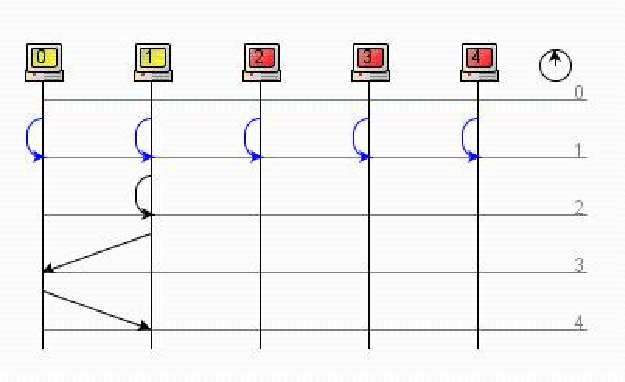
\includegraphics{images/p1ReadSeq.pdf}
	\caption{Bezeichnung der Abbildung}
	\label{a1}
\end{figure}

\begin{table} %[hbtp]
	\centering
		\begin{tabular}{l | l l l l}
		\textbf{Prozesse} & \textbf{Zeit} $\rightarrow$ \\
		\hline
			$P_{1}$ & $W(x)1$ \\
			$P_{2}$ & & $W(x)2$ \\
			$P_{3}$ & & $R(x)2$ & & $R(x)1$\\
			$P_{4}$ & & & $R(x)2$ & $R(x)1$\\
		\end{tabular}
	\caption{Bezeichnung der Tabelle}
	\label{t1}
\end{table}


\section{Mathematische Formel}\index{Formel}
Mathematische Formeln bzw. Formulierungen können sowohl im
laufenden Text (z.B. $y=x^2$) oder abgesetzt und zentriert im Text
erscheinen. Gleichungen sollten für Referenzierungen nummeriert
werden (siehe Formel \ref{gl-1}).
\begin{equation}
\label{gl-1}
e_{i}=\sum _{i=1}^{n}w_{i}x_{i}
\end{equation}

Entscheidungsformel:

\begin{equation}
\psi(t)=\left\{\begin{array}{ccc}
1 &  \qquad 0 <= t < \frac{1}{2} \\
-1 &  \qquad \frac{1}{2} <= t <1 \\
0 & \qquad sonst
\end{array} \right.
\end{equation}


Matrix:\index{Matrix}
\begin{equation}
A = \left(
\begin{array}{llll}
a_{11} & a_{12} & \ldots & a_{1n} \\
a_{21} & a_{22} & \ldots & a_{2n} \\
\vdots & \vdots & \ddots & \vdots \\
a_{n1} & a_{n2} & \ldots & a_{nn} \\
\end{array}
\right)
\end{equation}

Vektor:\index{Vektor} 

\begin{equation}
\overline{a} = \left(
\begin{array}{c}
a_{1}\\
a_{2}\\
\vdots\\
a_{n}\\
\end{array}
\right)
\end{equation}

\section{Sätze, Lemmas und Definitionen}\index{Satz}\index{Lemma}\index{Definition}

Sätze, Lemmas, Definitionen, Beweise,\index{Beweis} Beispiele\index{Beispiel} können in speziell dafür vorgesehenen Umgebungen erstellt werden.

\begin{definition}(Optimierungsproblem)

Ein \emph{Optimierungsproblem} $\mathcal{P}$ ist festgelegt durch ein Tupel
$(I_\mathcal{P}, sol_\mathcal{P}, m_\mathcal{P}, goal)$ wobei gilt

\begin{enumerate}
\item $I_\mathcal{P}$ ist die Menge der Instanzen,
\item $sol_\mathcal{P} : I_\mathcal{P} \longmapsto \mathbb{P}(S_\mathcal{P})$ ist eine Funktion, die jeder Instanz $x \in I_\mathcal{P}$ eine Menge zulässiger Lösungen zuweist,
\item $m_\mathcal{P} : I_\mathcal{P} \times S_\mathcal{P} \longmapsto \mathbb{N}$ ist eine Funktion, die jedem Paar $(x,y(x))$ mit $x \in I_\mathcal{P}$ und $y(x) \in sol_\mathcal{P}(x)$ eine
Zahl $m_\mathcal{P}(x,y(x)) \in \mathbb{N}$ zuordnet (= Maß für die Lösung $y(x)$ der Instanz $x$), und
\item $goal \in \{min,max\}$.
\end{enumerate}

\end{definition}

\begin{example} MINIMUM TRAVELING SALESMAN (MIN-TSP)
\begin{itemize}
\item $I_{MIN-TSP} =_{def}$ s.o., ebenso $S_{MIN-TSP}$
\item $sol_{MIN-TSP}(m,D) =_{def} S_{MIN-TSP} \cap \mathbb{N}^m$ 
\item $m_{MIN-TSP}((m,D),(c_1, \ldots , c_m)) =_{def} \sum_{i=1}^{m-1} D(c_i, c_{i+1}) + D(c_m,c_1)$ 
\item $goal_{MIN-TSP} =_{def} min$
\end{itemize}
\begin{flushright}
$\qed$
\end{flushright}
\end{example}

\begin{theorem} Sei $\mathcal{P}$ ein \textbf{NP}-hartes Optimierungsproblem.
Wenn $\mathcal{P} \in$ \textbf{PO}, dann ist \textbf{P} = \textbf{NP}.
\end{theorem}

\begin{proof} Um zu zeigen, dass \textbf{P} = \textbf{NP} gilt, genügt es
wegen Satz A.30 zu zeigen, dass ein einziges \textbf{NP}-vollständiges
Problem in \textbf{P} liegt. Sei also $\mathcal{P}'$ ein beliebiges \textbf{NP}-vollständiges Problem.

Weil $\mathcal{P}$ nach Voraussetzung \textbf{NP}-hart ist, gilt insbesondere
$\mathcal{P}' \leq_T \mathcal{P}_C$. Sei $R$ der zugehörige
Polynomialzeit-Algorithmus dieser Turing-Reduktion.
Weiter ist $\mathcal{P} \in$ \textbf{PO} vorausgesetzt, etwa vermöge eines
Polynomialzeit-Algorithmus $A$. Aus den beiden
Polynomialzeit-Algorithmen $R$ und $A$ erhält man nun
leicht einen effizienten Algorithmus für $\mathcal{P}'$: Ersetzt man
in $R$ das Orakel durch $A$, ergibt dies insgesamt eine polynomielle
Laufzeit. 
%\begin{flushright}
$\qed$
% \end{flushright}
\end{proof}

\begin{lemma} Aus \textbf{PO} $=$ \textbf{NPO} folgt \textbf{P} $=$ \textbf{NP}.
\end{lemma}

\begin{proof} Es genügt zu zeigen, dass unter der angegeben
Voraussetzung KNAPSACK $\in$ \textbf{P} ist.

Nach Voraussetung ist MAXIMUM KNAPSACK $\in$ \textbf{PO},
d.h. die Berechnung von $m^*(x)$ für jede Instanz $x$ ist
in Polynomialzeit möglich. Um KNAPSACK bei Eingabe
$(x,k)$ zu entscheiden, müssen wir nur noch $m^*(x) \geq k$
prüfen. Ist das der Fall, geben wir $1$, sonst $0$ aus. Dies
bleibt insgesamt ein Polynomialzeit-Algorithmus. 
\begin{flushright}
$\qed$
\end{flushright}
\end{proof}

\section{Fußnoten}

In einer Fußnote können ergänzende Informationen\footnote{Informationen die für die Arbeit zweitrangig sind, jedoch für den Leser interessant sein könnten.} angegeben werden. Außerdem kann eine Fußnote auch Links enthalten. Wird in der Arbeit eine Software (zum Beispiel Java-API\footnote{\url{http://java.sun.com/}}) eingesetzt, so kann die Quelle, die diese Software zur Verfügung stellt in der Fußnote angegeben werden.

\section{Literaturverweise}\index{Literatur}
Alle benutzte Literatur wird im Literaturverzeichnis angegeben\footnote{Dazu wird ein sogennanter bib-File, literatur.bib verwendet.}. Alle angegebene Literatur sollte mindestens einmal im Text referenziert werden\cite{Coulouris:02}.
\chapter{Beispielkapitel}

In diesem Kapitel wird beschrieben, warum es unterschiedliche Konsistenzmodelle\index{Konsistenzmodelle} gibt. Außerdem werden die Unterschiede zwischen strengen Konsistenzmodellen\index{Linearisierbarkeit} (Linearisierbarkeit, sequentielle Konsistenz)\index{sequentiell!Konsistenz} und schwachen Konsistenzmodellen\index{Konsistenz!schwach} (schwache Konsistenz, Freigabekonsistenz)\index{Freigabekonsistenz} erläutert. Es wird geklärt, was Strenge und Kosten (billig, teuer) in Zusammenhang mit Konsistenzmodellen bedeuten.

\section{Warum existieren unterschiedliche Konsistenzmodelle?}

Laut \cite{Malte:97} sind mit der\index{Replikation} Replikation von Daten immer zwei gegensätzliche Ziele verbunden: die Erhöhung der\index{Verfügbarkeit} Verfügbarkeit und die Sicherung der\index{Konsistenz} Konsistenz der Daten. Die Form der Konsistenzsicherung bestimmt dabei, inwiefern das eine Kriterium erfüllt und das andere dementsprechend nicht erfüllt ist (Trade-off zwischen Verfügbarkeit und der Konsistenz der Daten). Stark konsistente Daten sind stabil, das heißt, falls mehrere Kopien der Daten existieren, dürfen keine Abweichungen auftreten. Die Verfügbarkeit der Daten ist hier jedoch stark eingeschränkt. Je schwächer die Konsistenz wird, desto mehr Abweichungen können zwischen verschiedenen Kopien einer Datei auftreten, wobei die Konsistenz nur an bestimmten Synchronisationspunkten gewährleistet wird. Dafür steigt aber die Verfügbarkeit der Daten, weil sie sich leichter replizieren lassen.

Nach \cite{Mosberger:93} kann die Performanzsteigerung der schwächeren Konsistenzmodelle wegen der Optimierung\index{Optimierung} (Pufferung, Code-Scheduling, Pipelines) 10-40 Prozent betragen. Wenn man bedenkt, dass mit der Nutzung der vorhandenen Synchronisierungsmechanismen schwächere Konsistenzmodelle den Anforderungen der strengen Konsistenz genügen, stellt sich der höhere programmiertechnischer Aufwand bei der Implementierung der schwächeren Konsistenzmodelle als ihr einziges Manko dar.

In \cite{Cheriton:85} ist beschrieben, wie man sich Formen von DSM vorstellen könnte, für die ein beachtliches Maß an\index{Inkonsistenz} Inkonsistenz akzeptabel wäre. Beispielsweise könnte DSM verwendet werden, um die Auslastung von Computern in einem Netzwerk zu speichern, so dass Clients für die Ausführung ihrer Applikationen die am wenigsten ausgelasteten Computer auswählen können. Weil die Informationen dieser Art innerhalb kürzester Zeit ungenau werden können (und durch die Verwendung der veralteten Daten keine großen Nachteile entstehen können), wäre es vergebliche Mühe, sie ständig für alle Computer im System konsistent zu halten \cite{Coulouris:02}. Die meisten Applikationen stellen jedoch strengere Konsistenzanforderungen.

\section{Klassifizierung eines Konsistenzmodells}

Die zentrale Frage, die für die Klassifizierung\index{streng}\index{schwach} (streng oder schwach) eines Konsistenzmodells von Bedeutung ist \cite{Coulouris:02}: wenn ein Lesezugriff auf eine Speicherposition erfolgt, welche Werte von Schreibzugriffen auf diese Position sollen dann dem Lesevorgang bereitgestellt werden? Die Antwort für das schwächste Konsistenzmodell lautet: von jedem Schreibvorgang, der vor dem Lesen erfolgt ist, oder in der "`nahen"' Zukunft, innerhalb des definierten Betrachtungsraums, erfolgten wird. Also irgendein Wert, der vor oder nach dem Lesen geschrieben wurde.

Für das strengste Konsistenzmodell, Linearisierbarkeit (atomic consistency), stehen alle geschriebenen Werte allen Prozessoren sofort zur Verfügung: eine Lese-Operation gibt den aktuellsten Wert zurück, der geschrieben wurde, bevor das Lesen stattfand. Diese Definition ist aber in zweierlei Hinsicht problematisch. Erstens treten weder Schreib- noch Lese-Operationen zu genau einem Zeitpunkt auf, deshalb ist die Bedeutung von "`aktuellsten"' nicht immer klar. Zweitens ist es nicht immer möglich, genau festzustellen, ob ein Ereignis vor einem anderen stattgefunden hat, da es Begrenzungen dafür gibt, wie genau Uhren in einem verteilten System synchronisiert werden können.

Nachfolgend werden einige Konsistenzmodelle absteigend nach ihrer Strenge vorgestellt. Zuvor müssen wir allerdings klären, wie die Lese- und Schreibe-Operationen in dieser Ausarbeitung dargestellt werden.

Sei $x$ eine Speicherposition, dann können Instanzen dieser Operationen wie folgt ausgedrückt werden:
\begin{itemize}
	\item $R(x)a$ - eine Lese-Operation\index{Operation!Lese}, die den Wert $a$ von der Position $x$ liest.
	\item $W(x)b$ - eine Schreib-Operation\index{Operation!Schreib}, die den Wert $b$ an der Position $x$ speichert.
\end{itemize}

\section{Linearisierbarkeit\index{Linearisierbarkeit} (atomic consistency)}

Die Linearisierbarkeit im Zusammenhang mit DSM kann wie folgt definiert werden:
\begin{itemize}
	\item Die verzahnte Operationsabfolge findet so statt: wenn $R(x)a$ in der Folge vorkommt, dann ist die letzte Schreib-Operation, die vor ihr in der verzahnten Abfolge auftritt, $W(x)a$, oder es tritt keine Schreib-Operation vor ihr auf und $a$ ist der Anfangswert von $x$. Das bedeutet, dass eine Variable nur durch eine Schreib-Operation geändert werden kann.
	\item Die Reihenfolge der Operationen in der Verzahnung ist konsistent zu den \underline{Echtzeiten}\index{Echtzeiten}, zu denen die Operationen bei der tatsächlichen Ausführung aufgetreten sind.
\end{itemize}

Die Bedeutung dieser Definition kann an folgendem Beispiel (Tabelle \ref{tab:1}) nachvollzogen werden. Es sei angenommen, dass alle Werte mit $0$ vorinitialisiert sind.

\begin{table}
	\centering
		\begin{tabular}{l | l l l l}
			\textbf{Prozesse} & \textbf{Zeit} $\rightarrow$ & \\
			\hline
			$P_{1}$ & $W(x)1$ & & $W(y)2$ \\
			$P_{2}$ & & $R(x)1$ & & $R(y)2$ \\
		\end{tabular}
	\caption{Linearisierbarkeit ist erfüllt}
	\label{tab:1}
\end{table}

Hier sind beide Bedingungen erfüllt, da die Lese-Operationen den zuletzt geschriebenen Wert zurückliefern. Interessanter ist es, zu sehen, wann die Linearisierbarkeit verletzt ist.

\begin{table}
	\centering
		\begin{tabular}{l | l l l l}
		\textbf{Prozesse} & \textbf{Zeit} $\rightarrow$ \\
		\hline
		$P_{1}$ & $W(x)1$ & $W(x)2$ \\
		$P_{2}$ & & & \color{red} $R(x)0$ & \color{black} $R(x)2$ \\
		\end{tabular}
	\caption{Linearisierbarkeit ist verletzt, sequentielle Konsistenz ist erfüllt.}
	\label{tab:2}
\end{table}

In diesem Beispiel (Tabelle \ref{tab:2}) ist die Echtzeit-Anforderung verletzt, da der Prozess $P_{2}$ immer noch den alten Wert liest, obwohl er von Prozess $P_{1}$ bereits geändert wurde. Diese Ausführung wäre aber sequentiell konsistent (siehe kommender Abschnitt), da es eine Verzahnung der Operationen gibt, die diese Werte liefern könnte ($R(x)0$, $W(x)1$, $W(x)2$, $R(y)2$). 
\chapter{Zusammenfassung und Ausblick}

In diesem Kapitel soll die Arbeit noch einmal kurz zusammengefasst werden. Insbesondere sollen die wesentlichen Ergebnisse Ihrer Arbeit herausgehoben werden. Erfahrungen, die z.B. Benutzer mit der Mensch-Maschine-Schnittstelle gemacht haben oder Ergebnisse von Leistungsmessungen sollen an dieser Stelle präsentiert werden. Sie können in diesem Kapitel auch die Ergebnisse oder das Arbeitsumfeld Ihrer Arbeit kritisch bewerten. Wünschenswerte Erweiterungen sollen als Hinweise auf weiterführende Arbeiten erwähnt werden.
% ...
%--------------------------------------------------------------------------
\backmatter                        		% Anhang
%-------------------------------------------------------------------------
\bibliographystyle{geralpha}			% Literaturverzeichnis
\bibliography{literatur}     			% BibTeX-File literatur.bib


\end{document}
